%-*-    coding: UTF-8   -*-
% !TEX program = xelatex
\documentclass[UTF-8]{ctexart}
\usepackage{array}
\usepackage{graphicx}
\usepackage{subfigure}
\usepackage{amsmath}
\usepackage{amssymb}
\usepackage{tabularx}
\usepackage{multirow}
\usepackage[usenames,dvipsnames]{color}
\usepackage{framed}
\usepackage{listings}
\usepackage{hyperref}
\usepackage{verbatim}
\hypersetup{
	colorlinks=true,
	linkcolor=black,
	filecolor=black,      
	urlcolor=black,
	citecolor=black,
}
\usepackage{ulem}
\usepackage[cache=false]{minted}
\usepackage{geometry}
\geometry{a4paper,centering,scale=0.7}
\usepackage[format=hang,font=small,textfont=it]{caption}
\usepackage[nottoc]{tocbibind}

\definecolor{LightofNibel}{rgb}{0.6,0.85,0.95}
\pagecolor{white}

\title{\textbf{\huge LemonLime 用户手册}}
\author{\texttt{浮尘ii*, iotang}}
\date{}

\begin{document}
	\maketitle
	
	\begin{center}
	
\includegraphics[scale=0.5]{pics/icon.png}
	\end{center}
	\newpage
	
	\tableofcontents
	
	\newpage	
	
	\section{历史}
	
		\href{https://github.com/iotang/Project_LemonLime}{LemonLime} 项目是 \href{https://github.com/Dust1404/Project_LemonPlus}{LemonPlus} 的二次开发。
	
		~\\
	
		2011 年,Jia Zhipeng 开发完成了 Lemon,一个开源的评测工具。
		
		虽然我们并不知道他确切的动机,
		
		——是想弥补 Linux 下没有评测工具的缺陷,还是想造出一个 Cena 的对手,
		
		不管怎样,他的愿望达成了,Lemon 的历史也从此开始。
		
		现在(2020 年)他已经是一名得克萨斯大学奥斯汀分校的 2 年级博士生了,祝他的学业生涯顺利。\newline
		
		2018 年,在 浮尘ii* 的努力下,Lemon 进化为 LemonPlus。
		
		LemonPlus 成功兼容了 Qt 5,
		
		并且新增了适合新时代 OI 的功能,移除了一些不稳定的、过时的功能。
		
		奈何 OI 残酷,岁月更迁,物是人非,浮尘ii* 在 2019 年退役了,
		
		LemonPlus 的开发也相应地结束了。\newline
		
		2019 年,iotang 开始魔改 Lemon。
		
		起初,是想给 Lemon 增添一点用户体验——
		
		添加更多的颜色、优化界面,以及修改令人崩溃的重测逻辑,
		
		但是误打误撞地在 Github 上发现了 LemonPlus。
		
		可怜的 iotang 当时还不会用 Pull Request,所以 LemonLime 诞生了。
		
		LemonLime 继承了 LemonPlus 和 LemonMt(这个大概只有长郡人才会知道)的优点。\newline
		
		放眼望去,Lemon 的历史就像是传火。
		
		Lemon 开发要想继续,就必须要燃烧 Oier 的灵魂。
		
		就像是《精灵与萤火意志》的主角奥里那样,以自己的生命延续了精灵的纪元。\textcolor{white}{虽然这一作整个剧情就是一坨屎。}
		
		2020 年,随着政策巨变,iotang 也在退役的路上了。
		
		虽然退役并不代表开发停止,但是开发 Lemon 的热情将再也不能体会到了。
		
		也只能可惜 iotang 不够强了吧。\newline
		
		本篇用户手册是仿照 LemonPlus 的用户手册进行编写的。
		
	\newpage
	
	\section{Lemon 与开源意志}
		
		LemonLime 使用 GPL v3 协议。也就是说,LemonLime 是自由软件。\newline
		
		自由软件是什么?为什么 LemonLime 选择成为自由软件?
		
		自由软件意味着使用者有运行、复制、发布、研究、修改和改进该软件的自由。
		
		自由软件是权利问题,不是价格问题。
		
		要理解这个概念,你应该考虑“free”是“言论自由(free speech)”中的“自由”,
		
		而不是“免费啤酒(free beer)”中的“免费”。\newline
		
		更精确地说,自由软件赋予软件使用者四项基本自由:
		
		\begin{itemize}
			\item 不论目的为何,有运行该软件的自由(自由之零)。
			\item 有研究该软件如何工作以及按需改写该软件的自由(自由之一)。
			\item 有重新发布拷贝的自由,这样你可以借此来敦亲睦邻(自由之二)。
			\item 有向公众发布改进版软件的自由(自由之三),这样整个社群都可因此受惠。
		\end{itemize}
	
		不管是 Lemon,还是它的后继者 LemonPlus 和 LemonLime,
		
		都恪守着自由软件的意志。
		
		这是 LemonPlus 和 LemonLime 诞生的保障,
		
		也是 Lemon 不断延续自己的生命的保障。\newline
		
		\begin{center}
			
		Lemon,以及它的后继者们,拥抱开源。
		
		我们希望,Lemon 可以为全世界的 Oier 带来福祉。
		
		让我们一起,把 Lemon 变得更好。
		
		\end{center}
	
	\newpage
	
	\section{版本兼容性}
	
		LemonLime 近乎完全兼容 LemonPlus,出问题的地方在子任务依赖(为了支持 0 分测试点的让步,不过这个问题将会被解决)。不过这个问题在使用对应平台重新测试后就可以自动解决。
		
		LemonLime 完全兼容 Lemon。
	
	\newpage
	
	\section{安装}
	
		LemonLime 在上文中提及的\href{https://github.com/iotang/Project_LemonLime}{仓库地址}不仅用来存储源代码,也用来实时发布软件最新版本。
		
		\subsection{支持的系统}
		
			LemonLime 支持 Windows、Linux 以及 macOS。
			
		\subsection{安装方法}
			
			\subsubsection{Windows 和 macOS}
			
				在\href{https://github.com/iotang/Project_LemonLime/releases}{发行页面}下载相应的压缩包。
				
				不过如果你获得了源码,可以通过 QtCreator 来编译 LemonLime。
			
			\subsubsection{Linux}
			
				这里以 Manjaro 为例,毕竟 Linux 安装时几乎只有命令名字的区别。
				
				更多的系统请到 README.md 查看。
				
				首先你得安装一些依赖。
				
				\begin{lstlisting}[language=bash,frame=shadowbox,basicstyle=\ttfamily]
sudo pacman -S gcc make qt5-base
				\end{lstlisting}
				
				注意 Manjaro 的 gcc 包含了 g++。
				
				然后用某种途径获得源代码。比如使用 git:
				
				\begin{lstlisting}[language=bash,frame=shadowbox,basicstyle=\ttfamily]
git clone https://github.com/iotang/Project_LemonLime.git
				\end{lstlisting}
				
				进入源代码的目录。
				
				\begin{lstlisting}[language=bash,frame=shadowbox,basicstyle=\ttfamily]
cd 源代码的目录
				\end{lstlisting}
				
				然后依次执行:
				
				\begin{lstlisting}[language=bash,frame=shadowbox,basicstyle=\ttfamily]
g++ watcher_unix.cpp -o watcher_unix -O2
qmake lemon.pro
make
				\end{lstlisting}
				
				获得可执行文件 lemon。打开 lemon 就可以运行 LemonLime 了。
			
		\newpage
		
		\section{设置}
		
			LemonLime 没有设置编译器时(比如第一次运行)会自动弹出添加编译器的向导,具体的说明请看编译器配置一节。
		
			\subsection{常规设置}
			
				在工具菜单中选择“设置”,就能看到下图所示的对话框:
				
				\begin{center}
				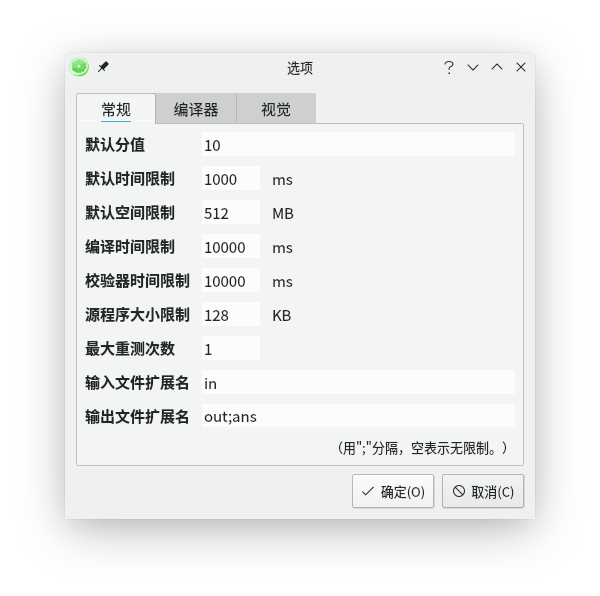
\includegraphics[scale=0.7]{pics/generalsettings.png}
				\end{center}
			
				各个设置意义如下:
				
				\begin{description}
					\item[默认分值] 新建一个测试点时的默认分值,默认为 10,可以设置的最大值为 10000000。
					\item[默认时间限制] 新建一个测试点默认的时间限制,默认为 1000 ms,可以设置的最大值为 86400000 ms,即 1 天。
					\item[默认空间限制] 新建一个测试点时默认的空间限制,默认为 512 MB,可以设置的最大值为 16777216 MB。
					\item[编译时间限制] 测试时允许编译器运行的最长时间,默认为 10000 ms,可以设置的最大值为 86400000 ms,即 1 天。
					\item[检验器时间限制] 对于使用自定义校验器的试题,测试时允许校验器运行的最长时间,默认为 10000 ms,可以设置的最大值为 86400000 ms,即 1 天。
					\item[源程序大小限制] 测试时可以接受的最大源程序大小,可以设置的最大值为 262144 KB,即 256 MB。(1 KB = 1024 B)
					\item[最大重测次数] 当测试某测试点时程序运行时间不超过时间限制的 1.1 倍,或超时不超过 100ms 时,LemonLime 会对该测试点进行重测。可以设置的最大值为 12。
					\item[输入、输出文件扩展名]  在自动添加试题时扫描的输入和输出文件的扩展名。如果有多个请用 \texttt{';'} 隔开。每种扩展名中只能包含英文字母和数字,Linux 平台下大小写是敏感的。注意这里的扩展名只供添加测试点时软件搜索文件使用,测试时并不会检查。
				\end{description}
		
			\subsection{编译器设置}
			
				点击上方的 “编译器” 选项卡就能进入编译器的配置。
				
				\begin{center}
					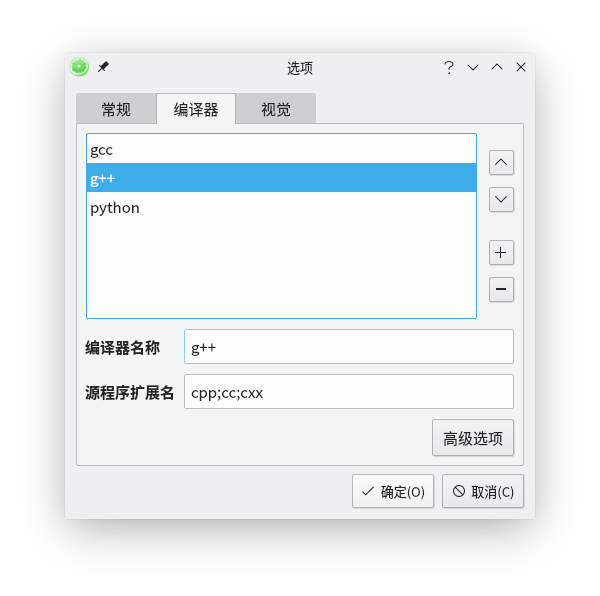
\includegraphics[scale=0.7]{pics/compilersettings.png}
				\end{center}
				
				按右边的加号就会出现添加编译器的向导,第一步是选择使用预置的编译器配置还是手动配置新的编译器。一般来说,用预置的配置就能够满足大多数需求,第一步只要在需要配置的编译器前打钩,进入下一步后就能看到选择路径的界面。
				
				\begin{center}
					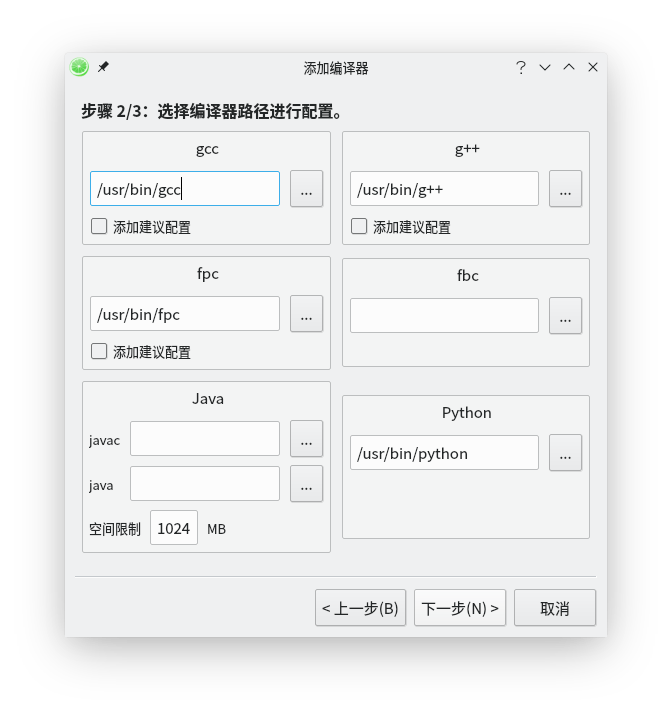
\includegraphics[scale=0.7]{pics/addcompiler.png}
				\end{center}
				
				\texttt{gcc}、\texttt{g++} 和 \texttt{fpc} 的建议配置中包含了不同标准和不同优化等级的组合。
				
				\texttt{Java} 的内存限制是由 Java 虚拟机限制的,你可以在之后的设置中选择不限制内存。
				
				最后一步会让你确认编译器路径是否设置正确。
				
				除了使用内置的六种编译器配置,你也可以选择手动配置新的编译器。
				
				\begin{center}
					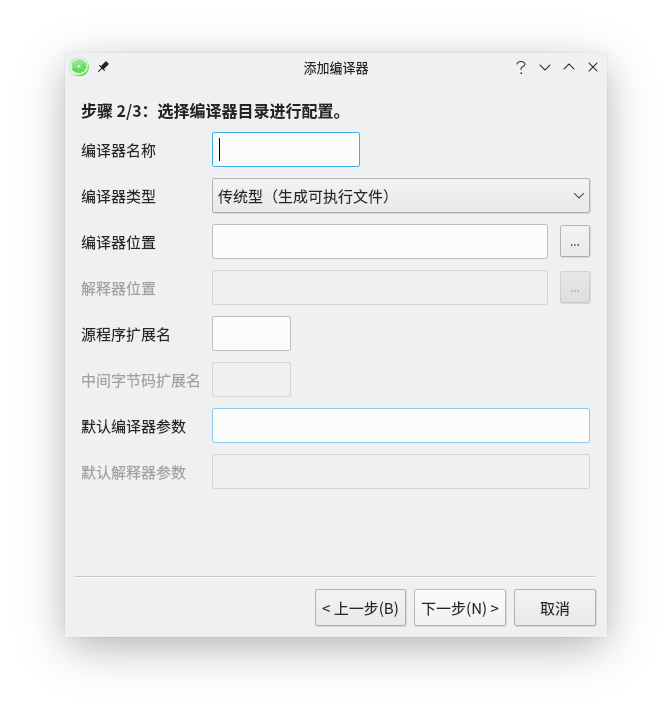
\includegraphics[scale=0.7]{pics/addcompiler2.png}
				\end{center}
				
				\begin{description}
					\item[编译器名称] 编译器在列表中显示的名称。
					\item[编译器类型] 总共有三种类型可选,括号里给出了相关解释。\texttt{C++}、\texttt{Java} 和 \texttt{Python} 分别是三种类型的典型代表。
					\item[编译器位置] 如果编译器的类型是传统型或需要编译的解释型,这里就要选择编译器的位置。对于传统型,编译器会将源代码直接转换成机器代码,而解释型的编译器会生成中间字节码。
					\item[解释器位置] 如果编译器的类型是解释型,就要选择解释器的位置。解释器用于执行中间字节码或直接解释执行源代码。
					\item[源程序扩展名] 用于判断哪些扩展名的源程序使用这个编译器编译,如果有多个扩展名请用 \texttt{';'} 隔开。
					\item[中间字节码扩展名] 解释型编译器生成的中间字节码的扩展名,例如 \texttt{Java} 的中间字节码扩展名为 \texttt{.class}。
					\item[默认编译器参数] 编译时传递给编译器的参数,其中用 \texttt{\%s} 表示不带扩展名的源程序文件名,\texttt{\%s.*} 表示带扩展名的源程序文件名。例如 \texttt{g++} 的编译参数为
					\begin{lstlisting}[frame=shadowbox,basicstyle=\ttfamily]
-o %s %s.* -lm
					\end{lstlisting}
					\item[默认解释器参数] 运行解释器时传递的参数,表示的方法同编译器参数。
				\end{description}
				
				向导完成后,我们再回到编译器管理的选项卡。
				
				如果要删除当前选择编译器,可以按右边的减号。
				
				右边的上下箭头是用来调整编译器优先级的。编译器的优先级是指:如果选手对于同一道题提交了多种扩展名的源程序,排在前面的编译器会被先考虑,同时在源程序扩展名中设置排在前面的扩展名会被先考虑。
				
				点击“高级选项”后可以进入下图的对话框来修改已有编译器的配置。
				
				\begin{center}
				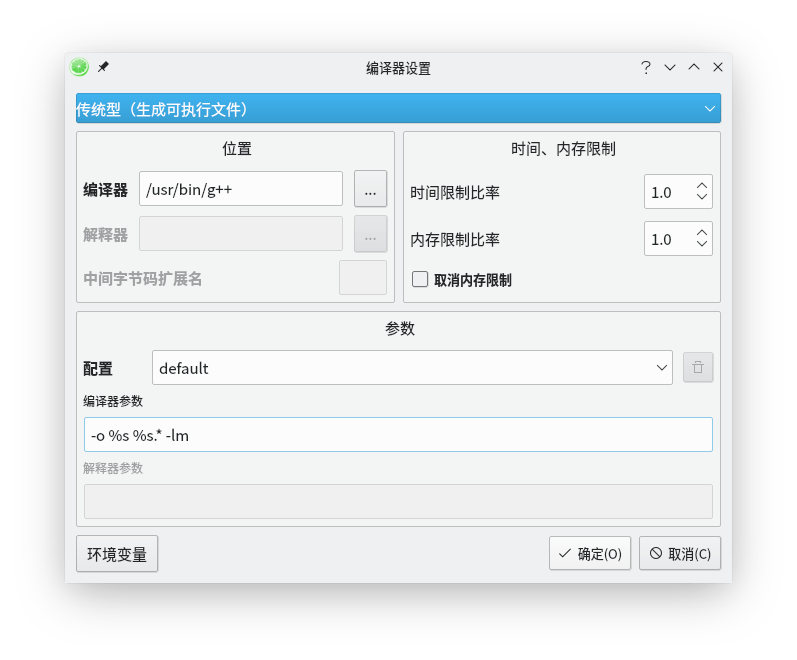
\includegraphics[scale=0.7]{pics/compilersettings2.png}
				\end{center}
				
				由于不同语言执行效率有差异,因此可以放宽特定语言的时间限制或空间限制,也就是将时间限制或空间限制乘上一个实数。你也可以选择直接取消空间限制。
				
				每个编译器都可以有多个配置,不同配置的编译参数或解释器运行参数不同,一般用于选择不同的优化开关。
				
				点击环境变量按钮可以设置编译器和程序运行时额外设置的环境变量,一般用于保证运行所需的动态链接库文件能被找到。
				
				
			\subsection{视觉设置}
				
				点击上方的 “视觉” 选项卡就能进入视觉配置。
				
				这个配置用于改善 LemonLime 的美观度以及提升定制性。
				
				\begin{center}
				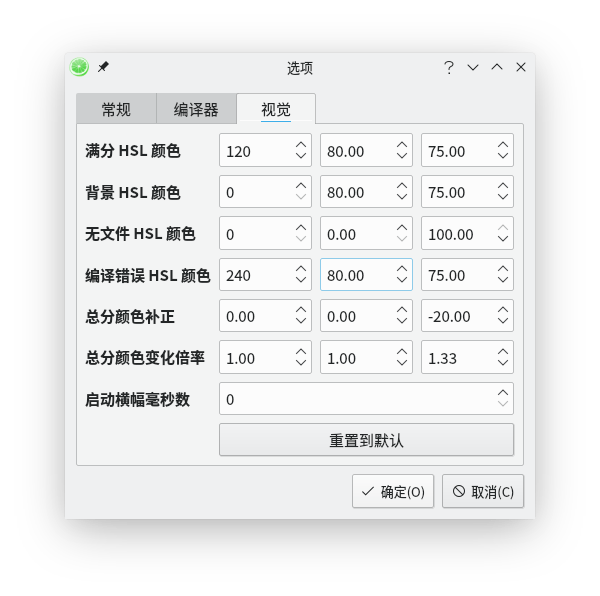
\includegraphics[scale=0.7]{pics/visualsettings.png}
				\end{center}
			
				\begin{description}
					\item[满分 HSL 颜色] 满分时的背景颜色,用 HSL 标准表示。从左往右第 1 个框是 H 值,范围为 0 到 719。第 2 个框是 S 值,范围为 0 到 100。第 3 个框是 L 值,范围为 0 到 100。
					\item[背景 HSL 颜色] 背景的颜色。不是满分的颜色为从背景 HSL 颜色到满分 HSL 颜色的根据得分与满分的比例的平滑变换。
					\item[无文件 HSL 颜色] 当某个选手某个题目找不到文件的时候的背景颜色。
					\item[编译错误 HSL 颜色] 当某个选手某个题编译错误的时候的背景颜色。
					\item[总分颜色补正] 总分一栏的颜色会对应地加上总分颜色补正的值。
					\item[总分颜色变化倍率] 总分一栏的颜色的变化倍率会对应地乘上总分颜色变化倍率的值。
					\item[启动横幅毫秒数] 启动时横幅显示的毫秒数。0 表示关闭。
					\item[重置到默认] 将以上所有值重置到默认。
				\end{description}
			
				你可以恰当地调整它们的值,来实现一些精彩的效果,比如实现暗色主题。
				
		\newpage
		
		
		\section{比赛}
		
			运行软件后会弹出 “欢迎” 对话框,可以选择打开已有的比赛或者新建比赛。如果关闭了这个对话框,也可以在文件菜单中选择打开或新建比赛。
			
			新建比赛的对话框如下图所示:
			
			\begin{center}
			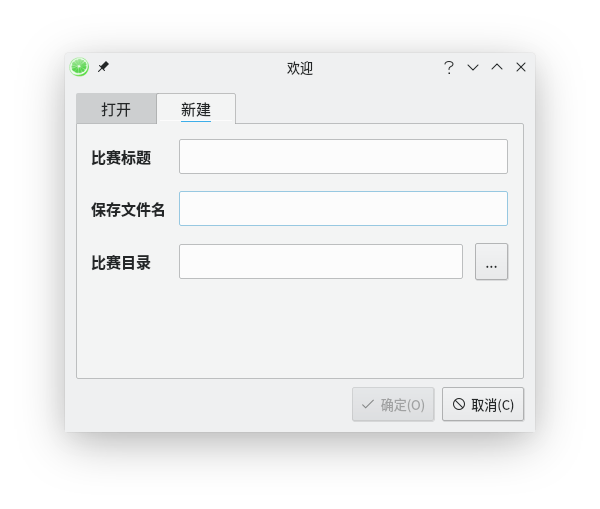
\includegraphics[scale=0.7]{pics/newcontest.png}
			\end{center}
			
			\begin{description}
				\item[比赛标题] 用来显示在软件标题栏上的比赛标题。
				\item[保存文件名] 保存比赛文件使用的文件名,这里输入的不需要附带扩展名。
				\item[比赛目录] 比赛相关文件的存储目录。  
			\end{description}
			
			点击确定后,软件会在制定的比赛目录下创建 \texttt{data} 和 \texttt{source} 目录,同时还有一个扩展名为 \texttt{cdf} 的文件名用来保存试题、选手信息。
			
			其中 \texttt{data} 下用来存放试题的数据、自定义的校验器、交互题的交互库、接口实现等文件,\texttt{source} 目录下存放每个选手的源程序或答案文件。
			
			\texttt{source} 目录下的每个文件夹代表一位选手,文件夹的名称为选手的名称。每位选手的文件夹是否需要对每个题目建立子文件夹可以在题目页面设置,见以下内容。
			
			你可以使用文件菜单栏中的 “打开当前比赛目录” 来打开当前比赛的目录。
			
			你还可以使用文件菜单栏中的 “更改比赛标题” 来更改当前比赛的标题。
			
		\subsection{添加新试题}
		
			建立好比赛后,在左边按鼠标右键就可以添加新的试题。然后在右边设置试题相关的信息。
			
			\begin{center}
			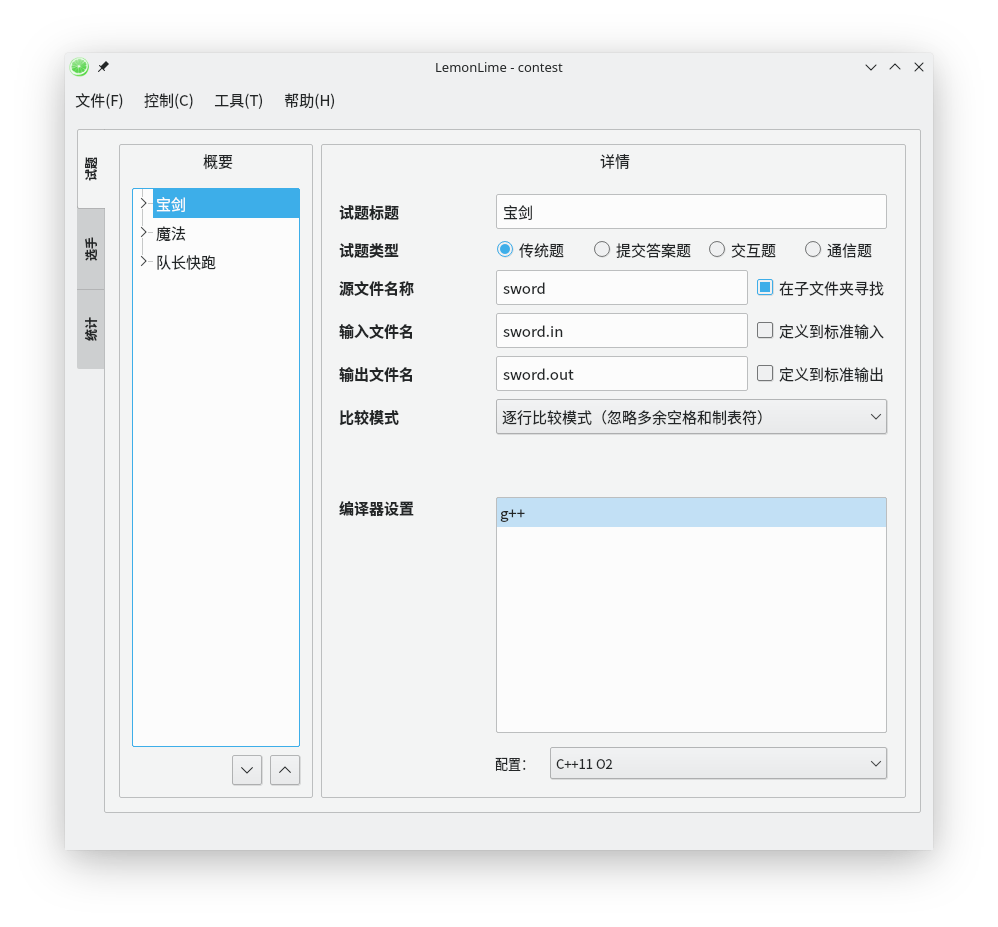
\includegraphics[scale=0.5]{pics/editproblem.png}
			\end{center}
			
			\begin{description}
				\item[概要下的一对箭头] 点击它们可以改变当前题目在列表的位置。
				\item[试题标题] 试题在列表中显示的名称。
				\item[试题类型] 试题的类型,目前可用的选择有传统题、提交答案题、交互题和通信题,其中交互型只支持 NOI 风格的 C++ 语言交互。
				\item[源文件名称] 源程序的文件名,注意不要带扩展名。并不一定要和试题标题相同。
				\item[在子文件夹中寻找] 若勾选,选手目录中需要为每个题单独建一个以源文件名称命名的文件夹,将源程序放在文件夹内;否则只需要将源程序放在选手目录下即可。
				\item[输入、输出文件名] 选手程序使用的输入输出文件名。
				\item[定义到标准输入、输出] 若勾选,则选手程序(交互题和通信题则是选手程序和接口文件编译出来的程序)会从标准输入读入数据(或向标准输出输出数据),不使用文件 IO。
				\item[比较模式] 比较选手输出和标准输出的方式,目前有五种方式:逐行比较模式、忽略多余空格和制表符的逐行比较模式(默认)、外部工具模式、实数比较模式和自定义校验器。
				
				逐行比较模式会一行一行比较选手的输出和标准输出是否相同,不同系统平台的换行符不同不会产生影响。
				
				逐行比较模式中也可以选择忽略多余的空格和制表符(这也是推荐的)。
				
				外部工具模式会调用 Linux 下的 \texttt{diff} 命令进行比较,但是小心 Windows 下可能没有 diff。
				
				实数比较模式会注意读取选手输出和标准输出中的每一个实数,分别比较误差是否在允许范围内,并且判断 \texttt{nan} 和 \texttt{inf}。
				
				自定义校验器 需要选择一个可执行文件作为校验器,具体的说明请参见下一个章节。
				\item[编译器设置] 为每个编译器选择配置,也就是选择相应的编译参数,默认会选择 \texttt{default} 配置。
				
				\item[选手答案文件扩展名] 这个只在提交答案题可见。对于提交答案题,选手提交的答案文件中,每个文件会和输入文件中去除扩展名后文件名一样的那个配对,这里可以设置选手提交的答案文件的扩展名,默认为 \texttt{out}。
				
				\item[交互库路径] 这个只在交互题可见。对于交互题,使用的交互库路径,通常为 \texttt{.h} 或 \texttt{.hpp} 文件。
				\item[交互库名称] 这个只在交互题可见。指选手需要引用的头文件名称。
				\item[接口实现(grader)路径] 这个只在交互题可见。一个实现交互库中的接口的文件。
				
				\item[源文件列表] 这个只在通信题可见。这个应该包含选手的所有要写的程序。可以通过右边的按钮来增删内容。
				\item[接口文件列表] 这个只在通信题可见。这个应该包含所有要用到的接口文件。可以通过右边的按钮来增删内容。注意这里的路径以 \texttt{data} 为根。
				\item[路径 / 文件名] 这个只在通信题可见。如果点击以上两项的“添加”,则会把这一栏的内容添加进对应项目。
			\end{description}
		
		
		\subsection{自定义校验器(SPJ)说明}
		
			自定义校验器需要为一个可执行文件,评测软件通过将一些参数传给校验器,使得校验器获得输出、输出文件等信息,然后将得分的结果写入指定文件中。
			
			评测软件会向校验器传入六个参数,按照顺序分别表示标准输入文件、选手输出文件、标准输入文件、本测试点满分、分数输出文件、额外信息文件。
			
			其中分数输出文件必须创建,需要向其中写入一个非负整数表示得分。
			
			额外信息文件可以不创建,如果创建了可以写入任何信息,这些信息会显示在结果中。
			
			\subsubsection{校验器实例}
			
				下面是一个例子。
				
				\begin{lstlisting}[language={C++},numbers=left,showspaces=false,showstringspaces=false,frame=shadowbox,basicstyle=\ttfamily]
#include<bits/stdc++.h>
using namespace std;

ifstream fin, fout, fstd;
ofstream fscore, freport;

inline void quit(int score, const char *msg)
{
	fscore << score;
	freport << msg;
	fin.close();
	fout.close();
	fstd.close();
	fscore.close();
	freport.close();
	exit(0);
}

int main(int argc, char **argv)
{
	fin.open(argv[1]);
	fout.open(argv[2]);
	fstd.open(argv[3]);
	int fullScore = atoi(argv[4]);
	fscore.open(argv[5]);
	freport.open(argv[6]);
	string ps, js;
	fout >> ps;
	fstd >> js;
	int P = js.length(), Q = ps.length(), K = 0;
	for (int i = 0; i < min(P, Q); i++)
		if (js[i] == ps[i]) K++;
	if (Q > P) K -= Q - P;
	if (K >= P)
	{
		quit(fullScore, "Success");
		return 0;
	}
	double ratio = 1.00 * K / P;
	if (ratio >= 0.6)
	{
		quit(0.4 * fullScore, "Great: 40%!");
		return 0;
	}
		
	quit(0, "Failed: @_@????????");
	
	return 0;
}
				\end{lstlisting}
		
			\subsubsection{使用 testlib}
			
				testlib 的使用说明可以在 \href{https://oi-wiki.org/intro/testlib/}{OI Wiki} 上见到。
				
				Lemon 所需的修改版 testlib 已经附在 LemonLime 源代码仓库中,
				
				名字为 \texttt{testlib\_for\_lemons.h}。
				
				注册 checker 只需要执行一句 \texttt{registerLemonChecker()} 即可。
				
				把上面的 spj 重写后如下所示:
		
				\begin{lstlisting}[language={C++},numbers=left,showspaces=false,showstringspaces=false,frame=shadowbox,basicstyle=\ttfamily]
#include<bits/stdc++.h>
#include"testlib_for_lemons.h"

using namespace std;

int main(int argc, char **argv)
{
	registerLemonChecker(argc, argv);
	int fullScore = perfectScore;
	string ps = ouf.readToken();
	string js = ans.readToken();
	int P = js.length(), Q = ps.length(), K = 0;
	for (int i = 0; i < min(P, Q); i++)
		if (js[i] == ps[i]) K++;
	if (Q > P) K -= Q - P;
	if (K >= P)
	{
		quitf(_ok, "Success");
		return 0;
	}
	double ratio = 1.00 * K / P;
	if (ratio >= 0.6)
	{
		quitp(0.4 * fullScore, "Great: 40%%!");
		return 0;
	}
	quitf(_wa, "Failed: @_@????????");
	
	return 0;
}
		
				\end{lstlisting}
				
				
		\subsection{关于非传统型试题}
				
			本节介绍了非传统型试题与传统题的区别以及测评逻辑。
				
			\subsubsection{提交答案题}
				
				提交答案题中,选手不需要提交源程序,只需要提交答案文件。
				
				所以测评中,不需要进行源程序的编译、运行,直接对答案进行判断即可。
				
				选手提交的答案文件名应与测试点配置中的输入文件相同(不包括扩展名),扩展名与题目配置的答案文件扩展名相同,软件将对选手提交的文件与测试点配置的答案文件以配置的比较模式进行比较。
				
			\subsubsection{交互题}
				
				只支持 NOI 风格的 C++ 语言交互。
				
				编译时将交互库拷贝至编译临时目录下并命名为交互库名称,将接口实现文件拷贝至目录下,进行双文件编译。
				
				对于交互库全部写在一个库文件中的题目(不推荐,选手可能会通过扫内存等方式获得信息),可以创建一个空的接口实现文件 \texttt{grader.cpp} 完成配置,不影响编译。
				
			\subsubsection{通信题}
			
				编译时将对应的所有文件拷贝至编译临时目录下进行多文件编译。
		
		\subsection{添加新测试点}
		
			在左边选中一道试题后,右键鼠标出现菜单,选择“添加测试点”即可添加一个新的测试点,右边会变成测试点设置界面。
			
			在输入文件名和输出文件名中输入内容后,点击“添加”按钮即可添加一组测试数据。这里的输入输出文件必须在 \texttt{data} 目录下,并且只要输入 \texttt{data} 目录内的相对路径即可,如下图所示:
			
			\begin{center}
			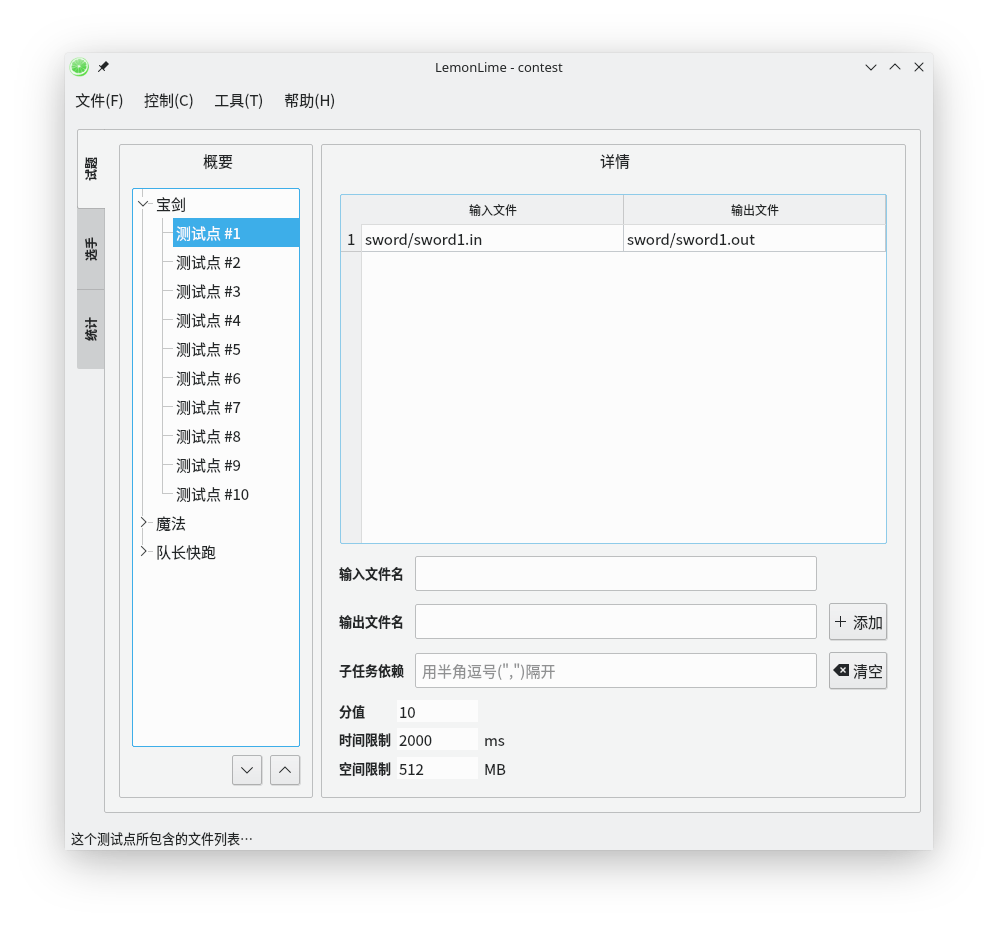
\includegraphics[scale=0.5]{pics/edittestcase.png}
			\end{center}
			
			一个测试点可以包含多组输入输出,最终一个测试点的得分为该测试点包含的所有测试数据中最低的得分。
			
			如果想要使用子任务依赖的话,对于测试点 $i$,请保证输入的子任务编号在 $[1, i - 1]$ 之间,多个依赖项之间用半角逗号(\texttt{,})隔开。子任务依赖的意思是这个测试点不会在被依赖的测试点中有错误(不是答案正确,且不是答案部分正确)的情况下测试。注意如果想清空的话,必须点击右边的“清空”按钮。
			
			如果要编辑输入输出文件名,直接在表格相应位置双击即可修改。
			
			选中一行或多行后按 \texttt{Delete} 键,即可删除对应的输入输出文件。
			
			在下面可以设置本测试点的分值、时间限制和空间限制。可以设置的最大分值为 10000000,最大时间限制为 86400000 ms(即 1 天),最大空间限制为 16777216 MB。
			
		\subsection{批量添加测试点}
		
			在左边选中一道试题后右键鼠标出现菜单,选择 “添加多组测试点…” 后会弹出一个向导,用来批量添加测试点。
			
			向导的第一步是设置每个测试点的分值、时间限制和空间限制,当然也可以添加完成后在编辑页面更改。
			
			第二步是设置如何匹配输入、输出文件名,这里需要会使用简单的正则表达式。
			
			输入、输出文件格式中可以使用 \texttt{<1>},\texttt{<2>},...,\texttt{<9>} 来表示一个正则表达式,然后在下面按右边的加号可以先见这样一个参数并指定参数代表的正则表达式。需要注意的是在输入文件格式和输出文件格式中,每个参数只能出现一次。
			
			对于所有参数匹配内容都相同的文件,会作为一组输入输出。
			
			对于打钩的参数匹配内容都相同的输入输出,会放在同一个测试点中。
			
			以一道捆绑测试的试题为例,在 \texttt{data} 下的 \texttt{sword} 文件夹里,有 \texttt{sword(x)-(y).in/out} 文件代表第 $x$ 个子任务的第 $y$ 个测试点的输入输出文件($x$ 和 $y$ 都是数字),那么匹配参数可以按照下图:
			
			\begin{center}
			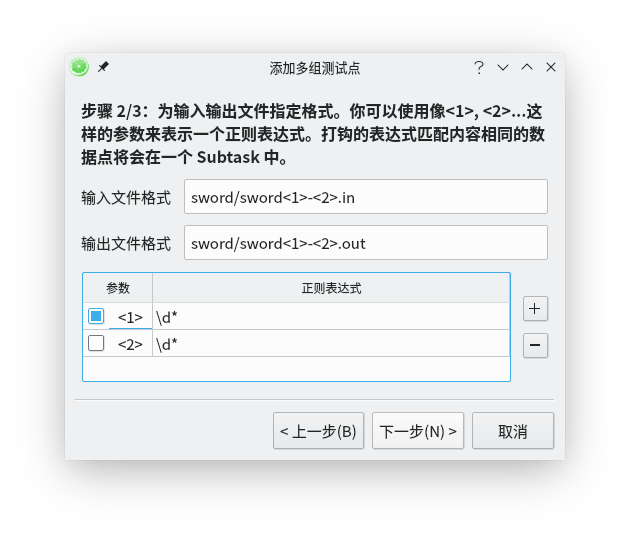
\includegraphics[scale=0.7]{pics/addtestcases.png}
			\end{center}
			
			注意:Windows 下文件夹分隔符为 \texttt{\textbackslash},Linux 下文件夹分隔符为 \texttt{/}。
			
			最后一步是预览结果,如果发现结果和预期的不同可以回到上一步修改参数。
				
		\subsection{自动添加试题}
		
			为了简化试题、测试数据的添加过程,Lemon 作者设计了自动添加试题功能。对于一道试题,如果希望能够自动添加,请在 \texttt{data} 目录中为这个试题创建一个文件夹,将相对应的数据文件放入文件夹中。然后再控制菜单中选择 “自动添加试题”,会出现一个对话框,给出找到的试题。
			
			可以设置每道试题所有测试点的总分值、所有测试点的时间限制和空间限制,确定后就会自动添加相应的试题。
			
			自动添加的试题默认作为传统型试题,添加后的试题标题和源程序名称都是对应试题的文件夹名称,输入输出文件分别再加上扩展名 \texttt{in} 和 \texttt{out}。
			
			数据文件的匹配方法是:根据设置中设定的输入输出文件扩展名,选出相应的文件,如果在设置中输入或输出文件扩展名为空,会自动将输入文件扩展名设置为 \texttt{in},输出文件扩展名设置为 \texttt{out;ans}。
			
			然后对于除扩展名外文件名相同的文件会被作为一组输入输出,并为这一组输入输出创建一个测试点,注意文件名的大小写是敏感的。
			
			用 “自动添加试题” 功能添加的试题,每个测试点只会有一组输入输出。
			
			每个测试点的分值会用设置的总分除以测试点个数,如果不能分配均匀的话,那么余下的点数会分配给后面的测试点。
			
			请尽量保证输入输出文件能够按上述方法唯一配对,否则产生的结果不可预料。
			
			其中可以设置的试题总分值最大为 10000000,最大时间限制为 86400000 ms(即 1 天),最大空间限制为 16777216 MB。
			
	\newpage
		
	\section{测试}
			
		点击“选手”选项卡,点击下面的“刷新”按钮后,就会根据 \texttt{source} 目录下的文件夹添加列表中不存在的选手,并从列表中删除已经从 \texttt{source} 目录中删除的选手。
		
		然后单击 “测试全部” 按钮就能开始测试。注意选手提交的程序名在 Linux 下是大小写敏感的。
		
		单击“测试未测试”按钮可以测试所有还没有测试的元素(即某个选手的某个题目)。
		
		选中一些元素后按“测试选中”按钮可以仅测试选中的部分。如果选中了某选手的排名、名称、总分、总用时、测试时间的其中某一个,那么将默认测试这个选手的所有题目。
		
		在控制菜单中还提供一键测试所有未找到文件的或者所有编译出错的记录。
		
		按 \texttt{Delete} 键或右键点击删除可以删除选中的选手。
		
		测试完成后通过在表头上单击可以按照相应的项目排序。
		
		双击一名选手可以查看详细的测试结果并对该选手的某一题进行重测。
		
		测试过程中会有 Subtask Skip,即对于一个测试点如果已经确定该测试点会得 0 分,则跳过这个测试点剩下的所有数据,可以大大减少捆绑测试的题目的测试时间。
		
		当然,LemonLime 还提供强制跳过某个题目的测试的功能。请不要在正式场合中使用。
		
		\subsection{测试情况对话框}
		
			\begin{center}
			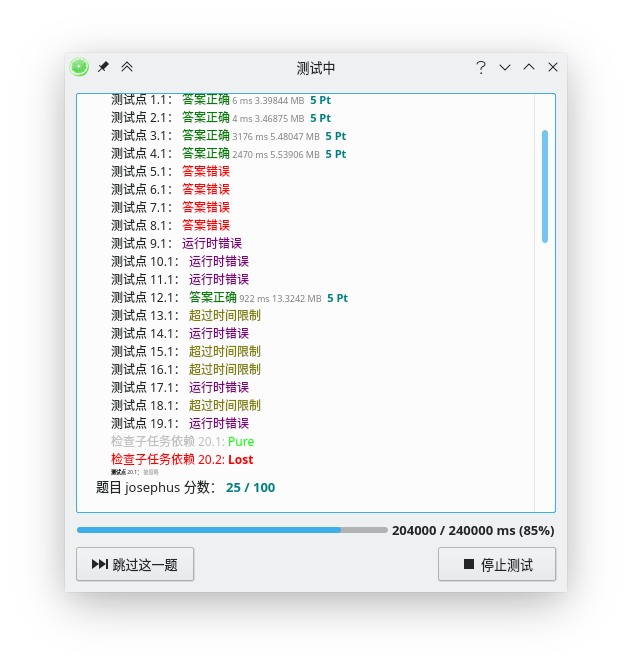
\includegraphics[scale=0.4]{pics/judgingdialog.png}
			\end{center}
		
			这个对话框会实时显示当前评测的情况。
			
			各种评测结果的字体颜色各不相同。
			
			如果选手在某一个测试点“答案正确”或者“答案部分正确”,那么会显示它的得分、用时和所使用的空间。
			
			进度条上会显示当前进度和总时间限制。
		
		\subsection{颜色}
		
			不同的选手的不同的题目会根据得分和评测状态呈现出不同的颜色。
			
			如果想改变颜色,可以到“设置”中改变。
		
		\subsection{整理文件}
		
			为每个选手的每一个文件创建它的子文件夹内的文件和子文件夹外的文件,无论它们以前是在子文件夹内还是子文件夹外,并且删除大部分无用文件。
			
			如果选手原本子文件夹内外都有文件,子文件夹外的那一个会被覆盖。
			
			注意这个功能对于提交答案题的支持还不够完善。最好在整理文件之前备份一份,以防不测。
		
		\subsection{跳过这一题}
		
			当你肯定某个选手是卡评测或者其它原因,或者这个题的评测结果无关紧要(比如自己自娱自乐的时候),那么可以点击“跳过这一题”。
			
			这会打断当前评测的题目,并跳过这道题之后的所有测试点。
			
			跳过的测试点会显示\texttt{超过时间限制}。
			
	\newpage
		
	\section{导出成绩}
	
		在 “控制” 菜单中选择 “导出成绩” 可以将结果导出成 HTML 文档或表格文件。
		
		推荐使用 HTML 格式,可以导出完整的结果信息,导出成表格的话只能导出选手总分和每道题的得分。
		
		表格有两种格式可以选择:csv 格式和 xls 格式(仅 Windows 可用并需要安装 Excel)。
		
		csv 格式是逗号分隔符,多数表格编辑软件都能查看。xls 格式的导出需要利用 ActiveX 调用 Excel,写入速度非常慢,除非特别需要,否则不推荐使用。
		
		在导出为 HTML 格式的时候,后缀(\texttt{.html} 和 \texttt{.htm})会影响内容。其中 \texttt{.html} 的内容会更加丰富,而 \texttt{.htm} 只提供基本内容,并且文件大小下降很多。
		
	\newpage
	
	\section{比赛统计}
	
		点击“统计”选项卡即可查看这场比赛的统计信息。
		
		\subsection{总览}
		
			这个部分显示了这场比赛的总体情况。
		
			\begin{center}
			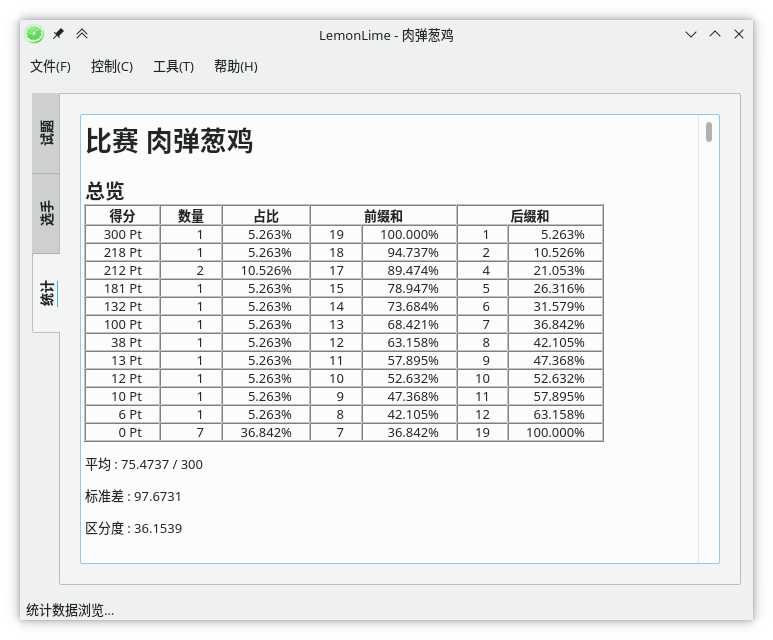
\includegraphics[scale=0.5]{pics/statistics.png}
			\end{center}
		
			你可以获得的信息有:
			
			\begin{itemize}
				\item 得到某个分数的选手人数以及比例,以及它的前缀和和后缀和。
				\item 这场比赛的平均分、分数的标准差和区分度。
			\end{itemize}
		
			其中,区分度是一个衡量本场比赛或某个题目的区分度的值。这个值仅供娱乐。
			
		
		\subsection{题目}
		
			每一个题目都有属于自己的一部分。这个部分显示了某个题目的情况。
			
			\begin{center}
			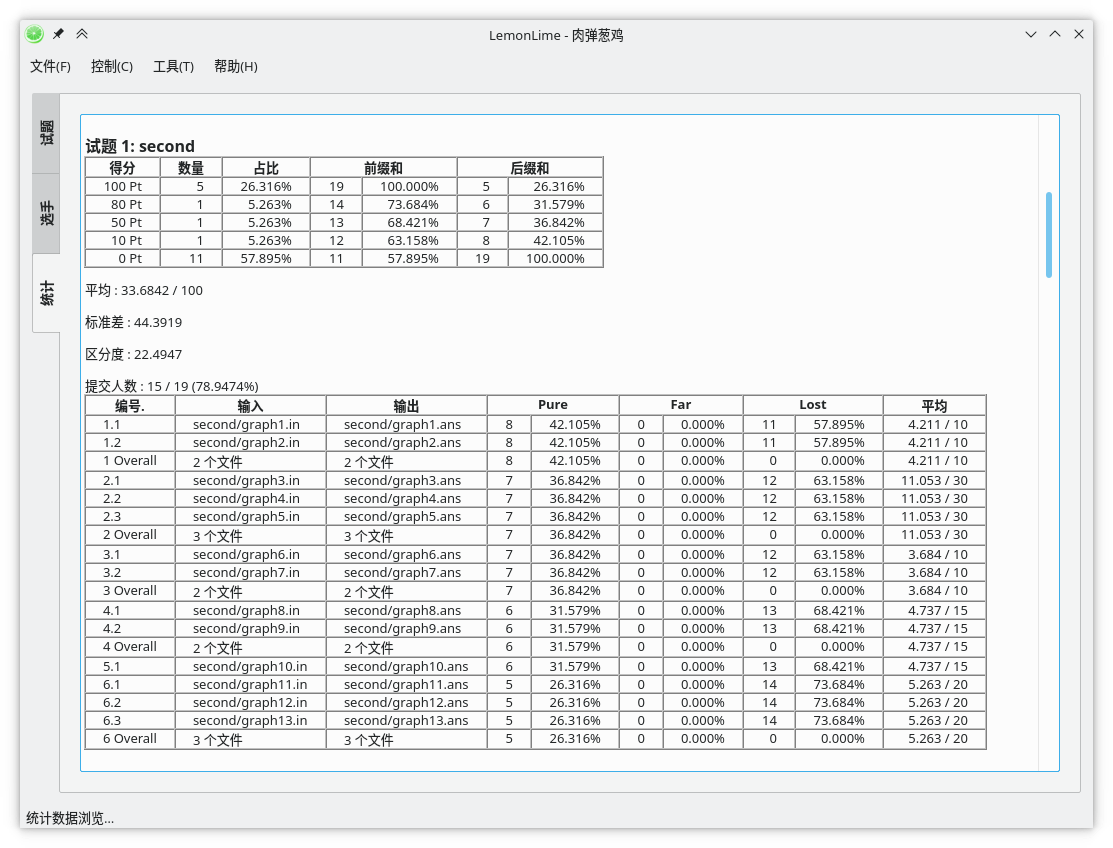
\includegraphics[scale=0.5]{pics/statistics2.png}
			\end{center}
		
			你可以获得的信息有:
		
			\begin{itemize}
				\item 得到某个分数的选手人数以及比例,以及它的前缀和和后缀和。
				\item 某个测试点的通过情况。
				\item 这个题目的平均分、分数的标准差、区分度和提交人数。
			\end{itemize}
		
		\subsection{导出统计信息}
	
			你可以使用控制菜单栏中的 “导出统计信息” 来导出当前比赛的导出统计信息到一个 HTML 文件。
			
			这个 HTML 文件的内容和 LemonLime 中的内容将完全一致。
	
	\newpage

	\section{常见问题及回答}
	
		在使用中出现任何问题,可以在 \href{https://github.com/iotang/Project_LemonLime}{Github 仓库}中的 Issue 提出。
		
		此节内容长期更新,更多问题欢迎提出。
		
		\subsection{测评时使用更多栈空间}
		
			Windows 平台下可以在 \texttt{g++} 编译时添加 \texttt{-Wl,--stack=2147483647} 命令来开启约 2048 MB 栈空间。
			
			Linux 平台下的栈空间限制和题目的内存限制相同。
			
	\newpage
			
\end{document}